\chapter{DESAIN DAN IMPLEMENTASI}
\label{chap:desainimplementasi}

Penelitian ini dilaksanakan sesuai sistem berikut dengan implementasinya. Desain sistem merupakan konsep dari pembuatan dan perancangan infrastuktur yang kemudian diwujudkan dalam bentuk blok diagram alur yang harus dikerjakan. Pada bagian implementasi merupakan pelaksanaan teknis untuk setiap blok pada desain sistem. Pada Gambar 3.1 menunjukan bagan umum metodologi sistem.

\begin{figure}[H]
  \centering
  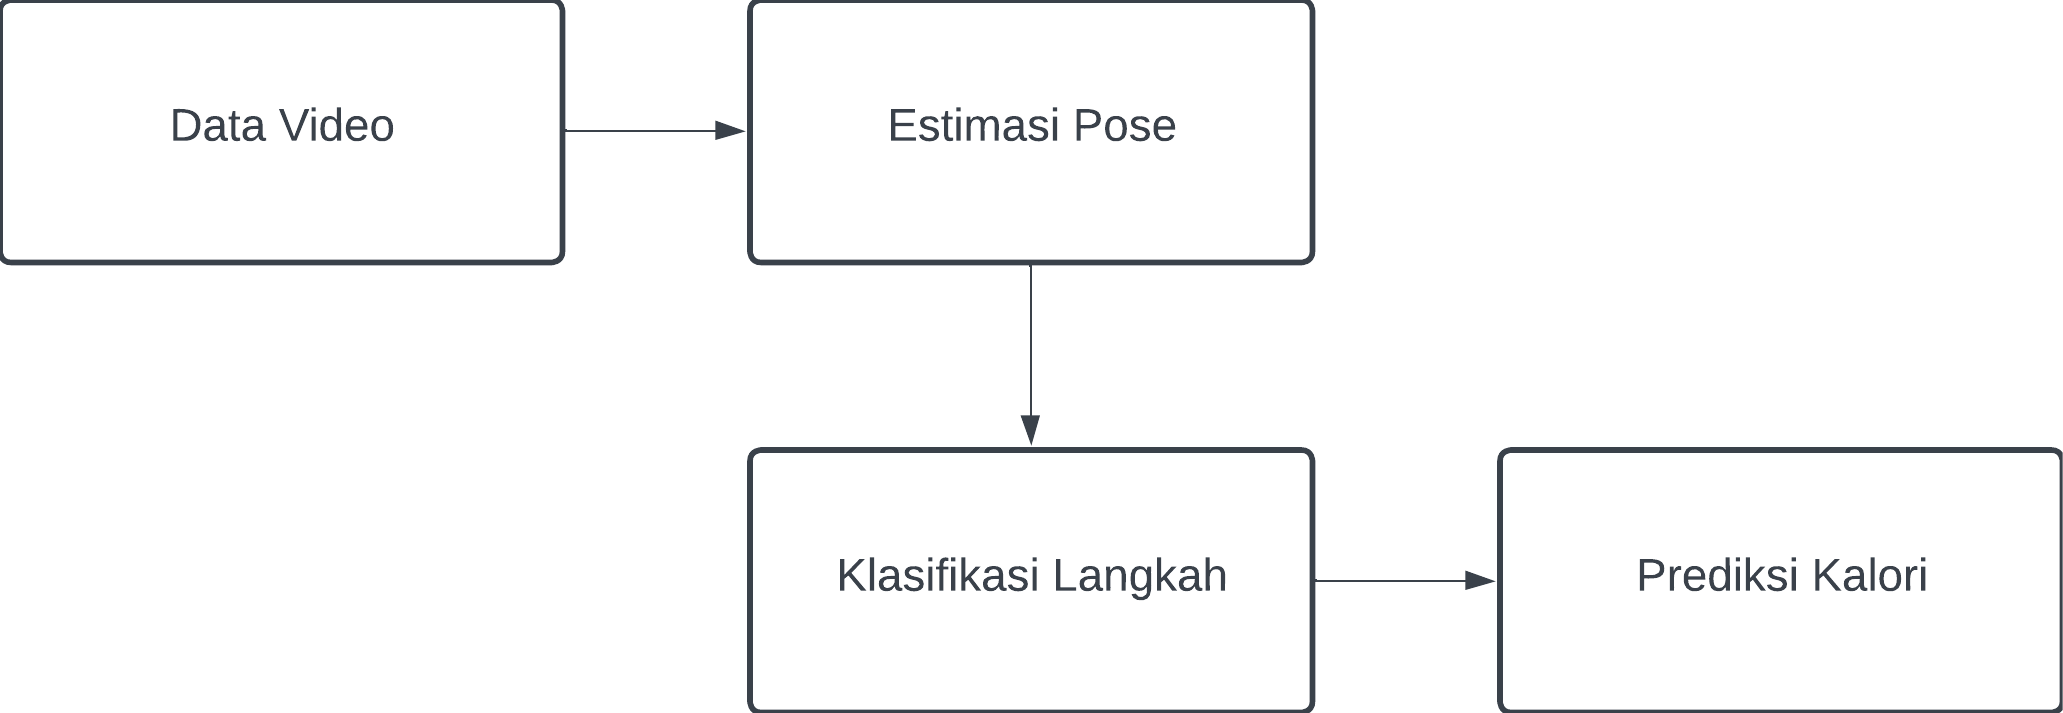
\includegraphics[scale=0.215]{gambar/blok diagram metodologi4.png}
  \caption{Blok Diagram Kerja Sistem}
  \label{fig:BlokDiagram}
\end{figure}

Berdasarkan Gambar \ref{fig:BlokDiagram} dalam menjelaskan alur kerja sistem yang digunakan dimulai dengan \emph{input} yang berupa data video menghasilkan beberapa data video yang akan digunakan dan diproses dengan melakukan estimasi pose dan klasifikasi langkah. Pada estimasi pose data video akan diestimasi pose untuk didapatkan hasil berupa dataset yang telah diekstrak fitur untuk dilakukan klasifikasi langkah. Klasifikasi langkah dilakukan dengan menggunakan model dari dataset yang dibuat dengan menggunakan arsitektur CNN untuk mendeteksi langkah. Hasil yang didapat dari proses klasifikasi langkah berupa banyak langkah dan waktu tempuh untuk dilakukan proses prediksi kalori. Prediksi kalori dilakukan dengan dua cara yaitu regresi dan perhitungan rumus. Hasil \emph{output} dari sistem ini adalah hasil prediksi kalori yang terbakar dari data video yang digunakan.

\section{Data Video}
\label{sec:PengambilanData}

Pada penelitian ini digunakan data berupa data video yang dilakukan pengambilan data dan diperoleh menggunakan kamera pada \emph{smartphone} yang akan direkam dan disimpan untuk kemudian akan digunakan pada proses yang dilakukan pada perangkat komputer/laptop atau dapat menggunakan kamera yang dimiliki oleh laptop atau kamera eksternal yang dihubungkan pada laptop ataupun komputer. Proses pengambilan data dilakukan dengan peraga melakukan aktivitas pada treadmill dengan ditampakkan secara jelas pada tampilan kamera. Setelah terdapat peraga dan tampak jelas pada tampilan maka data citra akan dilakukan pada tahap selanjutnya untuk dideteksi dan segmentasi pose seperti pada Gambar \ref{fig:DataVideo}.

\begin{figure}[H]
  \centering
  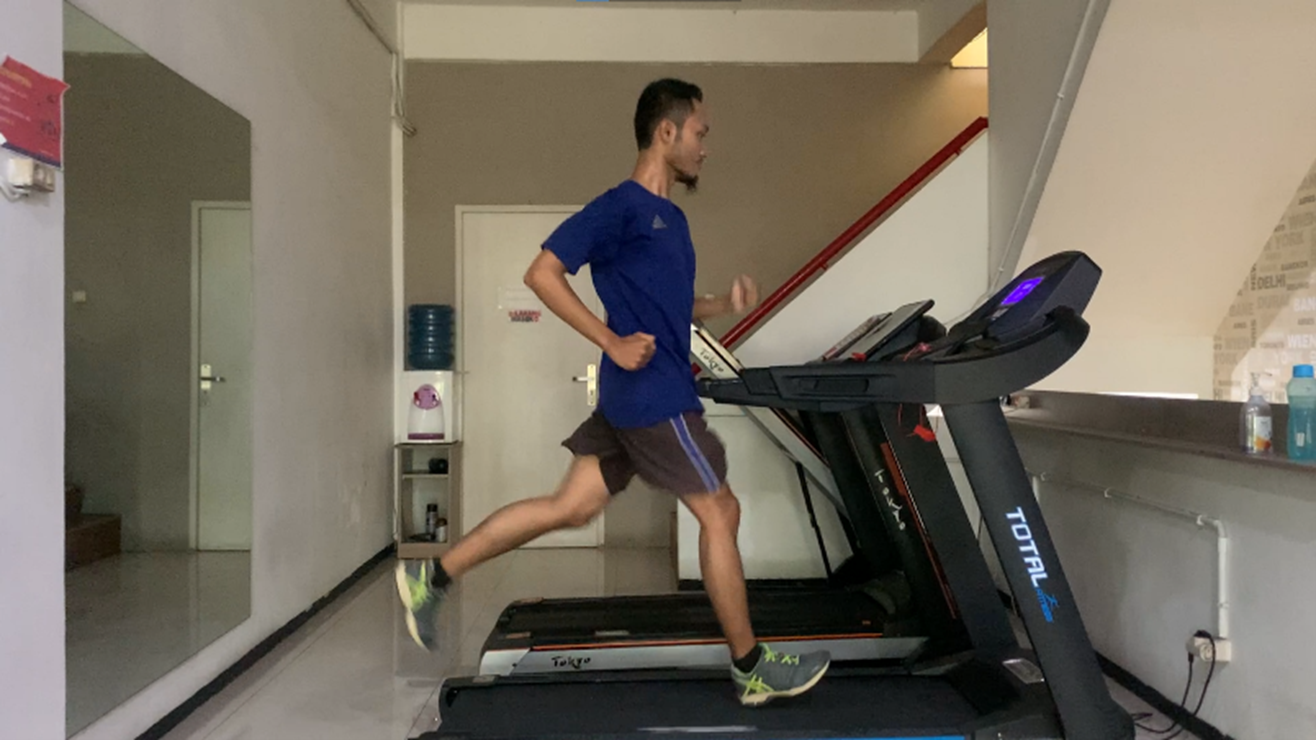
\includegraphics[scale=0.8]{gambar/pengambilan data.png}
  \caption{Proses pengambilan data}
  \label{fig:DataVideo}
\end{figure}

Data video yang digunakan pada penelitian ini berdasarkan pengambilan data video yang telah dilakukan. Pengambilan data dilakukan pada aktivitas yang dilakukan pada treadmill. Variasi yang digunakan pada data video yang digunakan berdasarkan variasi kecepatan dan hasil kalori yang terbakar. Tabel \ref{tb:DatasetVideo} menunjukkan data video berdasarkan variasi yang digunakan.

\begin{longtable}{|c|c|c|}
  \caption{Data video berdasarkan pengambilan data}
  \label{tb:DatasetVideo}  \\
  \hline
  \rowcolor[HTML]{C0C0C0}
  \textbf{Percobaan} & \textbf{Kecepatan} & \textbf{Kalori Terbakar} \\
  \hline
  1     & 3     & 10   \\
  \hline
  2     & 6     & 10   \\
  \hline
  3     & 9     & 20   \\
  \hline
  4     & 12    & 20   \\
  \hline
  5     & 8     & 20   \\
  \hline
  7     & 12    & 20   \\
  \hline
\end{longtable}


\section{Estimasi Pose}
\label{sec:EstimasiPose}

Estimasi dari hasil citra untuk dapat mengetahui bentuk postur tubuh manusia menggunakan Python dengan \emph{library} OpenCV yaitu MediaPipe. Metode yang digunakan pada MediaPipe menggunakan estimasi pose untuk mendeteksi postur tubuh. Segementasi dilakukan dengan cara peraga melakukan aktivitas \emph{jogging} pada treadmill dengan menentukan pose melangkah ataupun berlari sesuai dengan olahraga yang akan diteliti. Data yang diproses merupakan data yang telah dilakukan perekaman pada proses pengambilan data dengan menggunakan video yang telah direkam sebelumnya menggunakan alat perekam. Hasil video yang memperlihatkan seseorang dalam keadaan berolahraga pada treadmill melakukan aktivitas berjalan atau berlari akan diproses dalam tahap ini untuk dilakukan estimasi pose. Estimasi pose menggunakan model Estimasi yang sudah ada yaitu Mediapipe. Hasil estimasi dari model Mediapipe berupa kerangka yang menyesuaikan bentuk tubuh yang diestimasi dari data video yang dimiliki.

Dalam penelitian ini yang berfokuskan pada proses deteksi langkah pada tubuh bagian bawah seperti kaki menyebabkan perlunya pemodelan ulang dan melakukan proses modifikasi pada hasil estimasi model Mediapipe. Dengan begitu proses modifikasi yang dilakukan adalah dengan mengambil kerangka bagian kaki dengan memberikan warna yang berbeda untuk hasil estimasi kaki bagian kiri dan kanan. Proses estimasi pose pada kaki yang dilakukan akan digunakan dalam proses selanjutnya dalam penelitian ini yang digambarkan pada gambar yang terdapat pada Gambar \ref{fig:DeteksiEstimasi}.

\begin{figure}[H]
  \centering
  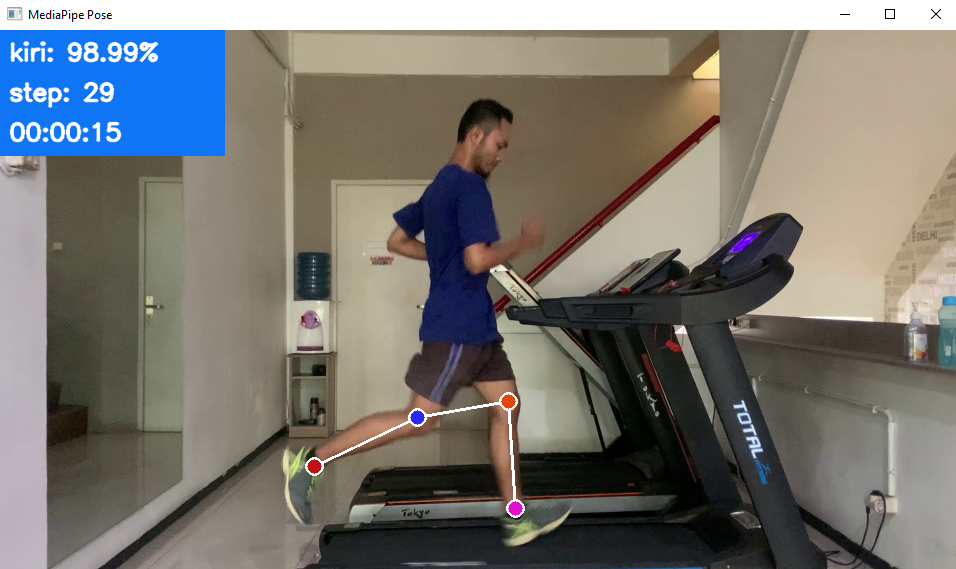
\includegraphics[scale=0.45]{gambar/deteksi pose.png}
  \caption{Estimasi pose dengan MediaPipe}
  \label{fig:DeteksiEstimasi}
\end{figure}

\subsection{\emph{Preprocessing} Data}
\label{subsec:PreProcessingData}

Hasil estimasi pose dengan bentuk kerangka pada kaki sesuai dengan data video dilakukan tahap \emph{preprocessing}. \emph{Preprocessing} data dilakukan sebagai proses untuk mempersiapkan data dari input yang digunakan untuk kemudian dilakukannya proses pembuatan model dalam tahap \emph{training}. Terdapat beberapa tahapan yang dilakukan pada \emph{preprocessing} data untuk kemudian akan didapatkan dataset yang akan dapat digunakan untuk melakukan pembuatan model dengan proses \emph{training}. Setiap data video yang akan digunakan dalam proses ini akan dilakukan ekstrak dari data video menjadi gambar. Data video yang memiliki resolusi sebesar 1920 x 1080 dengan 25 FPS akan diubah dan diekstrak menjadi satuan gambar untuk digunakan sebagai dataset melalui proses \emph{preprocessing} data. Dengan resolusi data demikian akan menghasilkan 25 gambar atau \emph{frame} setiap satu detik dari video tersebut. Hasil ekstrak gambar dalam \emph{preprocessing} data ini akan kemudian dilanjutkan dalam proses untuk membuat dataset untuk kemudian digunakan dalam proses \emph{training} menjadi model.

\subsection{Ekstrak Fitur}
\label{subsec:AugmentasiData}

Pada proses estimasi pose didapat hasil estimasi pada data video berupa kerangka pada kaki yang menyesuaikan bentuk tubuh yang sedang ditampilkan. Setelah dapat diestimasi dengan baik menggunakan model Mediapipe dan dimodifikasi untuk dapat terfokus pada bagian kaki, dilakukan proses ekstrak fitur. Ekstrak fitur dilakukan sebagai proses untuk mengubah atau memodifikasi gambar agar dapat dengan mudah diproses dalam tahap \emph{training}. Proses ini juga akan dapat membantu dalam meningkatkan akurasi dari model yang akan digunakan nanti karena data telah diproses dan dimodifikasi agar memiliki data-data tambahan yang akan berguna dalam tahap \emph{training}. Data dari proses estimasi pose akan dilakukan proses pemindahan hasil estimasi kerangka ke dalam gambar baru dengan penyesuaian yang akan digeneralisasikan terhadap semua data yang didapat. 

Proses dimulai dengan menentukan posisi kerangka dari data video asli untuk kemudian akan dipindahkan ke gambar baru. Dalam melakukan menentukan posisi kerangka dilakukan dengan estimasi menggunakan bingkai yang menyesuaikan posisi keseluruhan kerangka yang dapat dilihat pada Gambar \ref{fig:PreProcessing1}. Setelah bingkai menyesuaikan posisi kerangka maka akan dipindahkan pada gambar dengan latar belakang hitam yang berisikan hanya kerangka dari hasil estimasi sesuai dengan bingkai. Proses melakukan pemindahan hasil estimasi ke dalam gambar dengan latar belakang hitam dapat ditunjukan pada gambar Gambar \ref{fig:PreProcessing2}. Kemudian gambar akan dilakukan generalisasi terhadap ukuran yang berisikan hanya hasil estimasi sesuai bingkai untuk mempermudah dalam proses selanjutnya dengan membuat ukuran gambar seragam dalam bentuk persegi.

\begin{figure}[H]
  \centering
  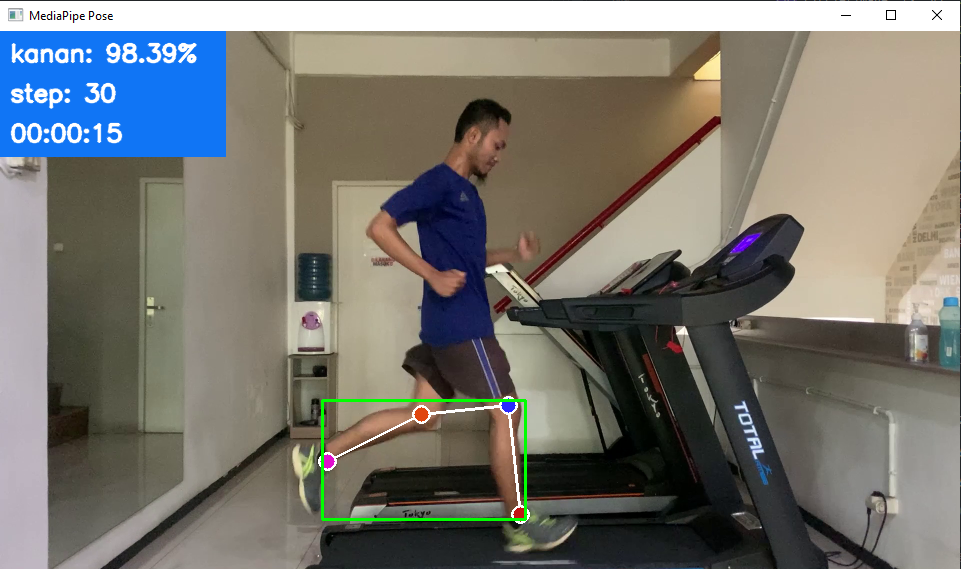
\includegraphics[scale=0.48]{gambar/deteksi pose2.png}
  \caption{\emph{Preprocessing} hasil estimasi pose dengan bingkai}
  \label{fig:PreProcessing1}
\end{figure}

\begin{figure}[H]
  \centering
  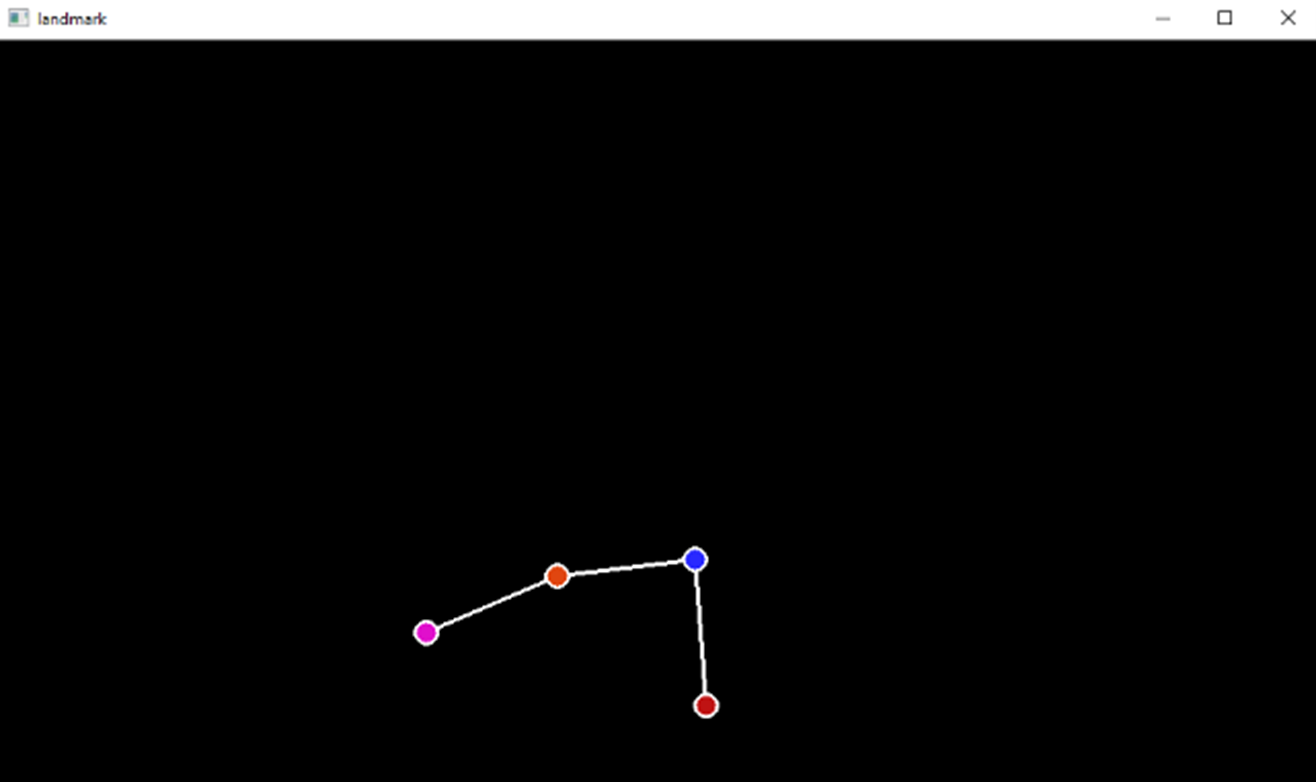
\includegraphics[scale=0.8]{gambar/deteksi pose3.png}
  \caption{\emph{Preprocessing} hasil estimasi pose pada latar belakang hitam}
  \label{fig:PreProcessing2}
\end{figure}

\subsection{Pelabelan Objek}
\label{subsec:PelabelanObjek}

Hasil dari proses ekstrak fitur dengan melakukan pemindahan hasil estimasi ke dalam gambar baru yang telah disesuaikan akan diproses menjadi sebuah dataset. Pelabelan objek diperlukan untuk dapat memberikan informasi nama kelas dari objek yang akan dideteksi pada penelitian ini. Proses pada pelabelan objek ini dilakukan setelah didapatkan proses dalam \emph{preprocessing} dengan mengekstrak data video menjadi gambar dan dilakukan proses ekstrak fitur dari setiap data gambar yang didapat. Kemudian dari hasil ekstrak fitur dengan memiliki hasil gambar kerangka berdasarkan hasil deteksi dikelompokkan pada kategori atau kelas yang berbeda. Pada penelitian ini proses deteksi yang diinginkan adalah dapat menentukan proses aktivitas melangkah atau berlari dengan mengetahui kaki kanan atau kiri yang sedang berada di depan. Dengan begitu kelas yang dimiliki pada dataset yang akan dibuat dengan terdapat dua label atau kelas yaitu kanan dan kiri. Hasil ekstraksi dan ekstrak fitur yang dilakukan berdasarkan kelas yang diinginkan dapat dilihat untuk kelas kanan pada Gambar \ref{fig:KelasKanan} dan untuk kelas kiri pada Gambar \ref{fig:KelasKiri}. Dari setiap gambar yang telah dilakukan ekstraksi fitur dilakukan pemberian label sesuai dengan kelas yang akan digunakan. Hasil pelabelan objek gambar tersebut ditunjukkan pada Tabel \ref{tb:HasilAnotasi}.

\begin{figure}[H]
  \centering
  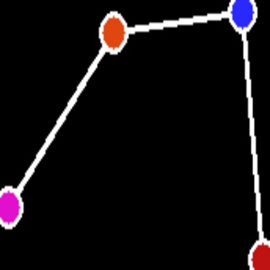
\includegraphics[scale=0.8]{gambar/dataset kanan.png}
  \caption{Hasil \emph{preprocessing} untuk kelas kanan}
  \label{fig:KelasKanan}
\end{figure}

\begin{figure}[H]
  \centering
  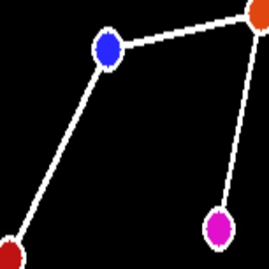
\includegraphics[scale=0.8]{gambar/dataset kiri.png}
  \caption{Hasil \emph{preprocessing} untuk kelas kiri}
  \label{fig:KelasKiri}
\end{figure}

\begin{longtable}{|c|c|}
  \caption{Hasil anotasi dari pelabelan objek}
  \label{tb:HasilAnotasi}  \\
  \hline
  \rowcolor[HTML]{C0C0C0}
  \textbf{Kelas} & \textbf{Jumlah Anotasi}  \\
  \hline
  Kanan           & 888    \\
  \hline
  Kiri            & 843    \\
  \hline
  \textbf{Total}  & \textbf{1.731}  \\
  \hline
\end{longtable}


\subsection{Dataset}
\label{subsec:Dataset}

Dataset yang digunakan pada penelitian ini berdasarkan hasil dari data video yang dimiliki dengan mengambil sampel pada proses pengambilan data. Kemudian dilakukan proses \emph{preprocessing} dengan melakukan ekstraksi gambar, augmentasi data, dan pelabelan objek yang akan disimpan keseluruhan data yang dimiliki berdasarkan kelas untuk menjadi dataset yang akan digunakan pada penelitian ini. Dataset yang telah dimiliki pada penelitian ini berupa data gambar berisikan bentuk kerangka dari hasil deteksi dengan model Mediapipe yang telah dimodifikasi dan digeneralisasi untuk ukuran gambar. Hasil dari dataset yang akan digunakan untuk dataset kelas kanan ditunjukkan pada Gambar \ref{fig:DatasetKanan} dan untuk dataset kelas kiri ditunjukkan pada Gambar \ref{fig:DatasetKiri}.

\begin{figure}[H]
  \centering
  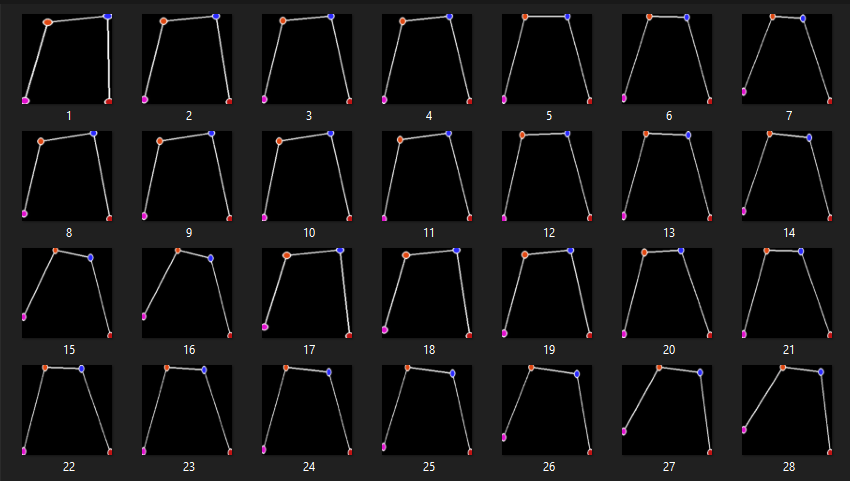
\includegraphics[scale=0.45]{gambar/folder dataset kanan.png}
  \caption{Dataset untuk kelas Kanan}
  \label{fig:DatasetKanan}
\end{figure}

\begin{figure}[H]
  \centering
  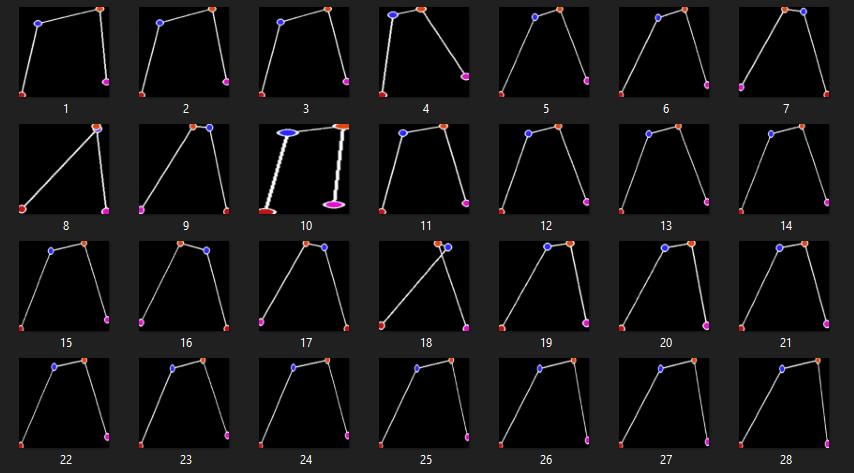
\includegraphics[scale=0.45]{gambar/folder dataset kiri.png}
  \caption{Dataset untuk kelas Kiri}
  \label{fig:DatasetKiri}
\end{figure}


\section{Klasifikasi Langkah}
\label{sec:KlasifikasiLangkah}

Dataset yang telah dimiliki maka kemudian dilakukan \emph{training} untuk memperoleh model deteksi. Model deteksi dari dataset akan digunakan untuk melatih model dari sebuah algoritma pada \emph{Machine Learning}. Dalam melakukan klasifikasi menggunakan \emph{Convolutional Neural Networks} (CNN). Proses \emph{training} ini bertujuan agar nantinya komputasi yang dilakukan dalam proses deteksi akan dapat diolah berdasarkan akuisisi data citra yang ingin dideteksi menjadi bentuk atau pola pemahaman yang diinginkan. Hasil \emph{training} akan didapatkan model yang digunakan untuk melakukan klasifikasi atas dataset yang dimiliki yaitu terdapat dua kelas atau label untuk dapat diklasifikasikan menjadi kaki kanan dan kiri. Klasifikasi dalam menentukan aktivitas yang digunakan pada penelitian ini adalah dapat mengetahu langkah dari seseorang yang berjalan atau berlari. Hasil klasifikasi dari model yang telah dibuat untuk menentukan hasil deteksi untuk kelas kanan ditunjukkan pada Gambar \ref{fig:KlasifikasiKanan} dan hasil deteksi untuk kelas kiri ditunjukkan pada Gambar \ref{fig:KlasifikasiKiri}.

\begin{figure}[H]
  \centering
  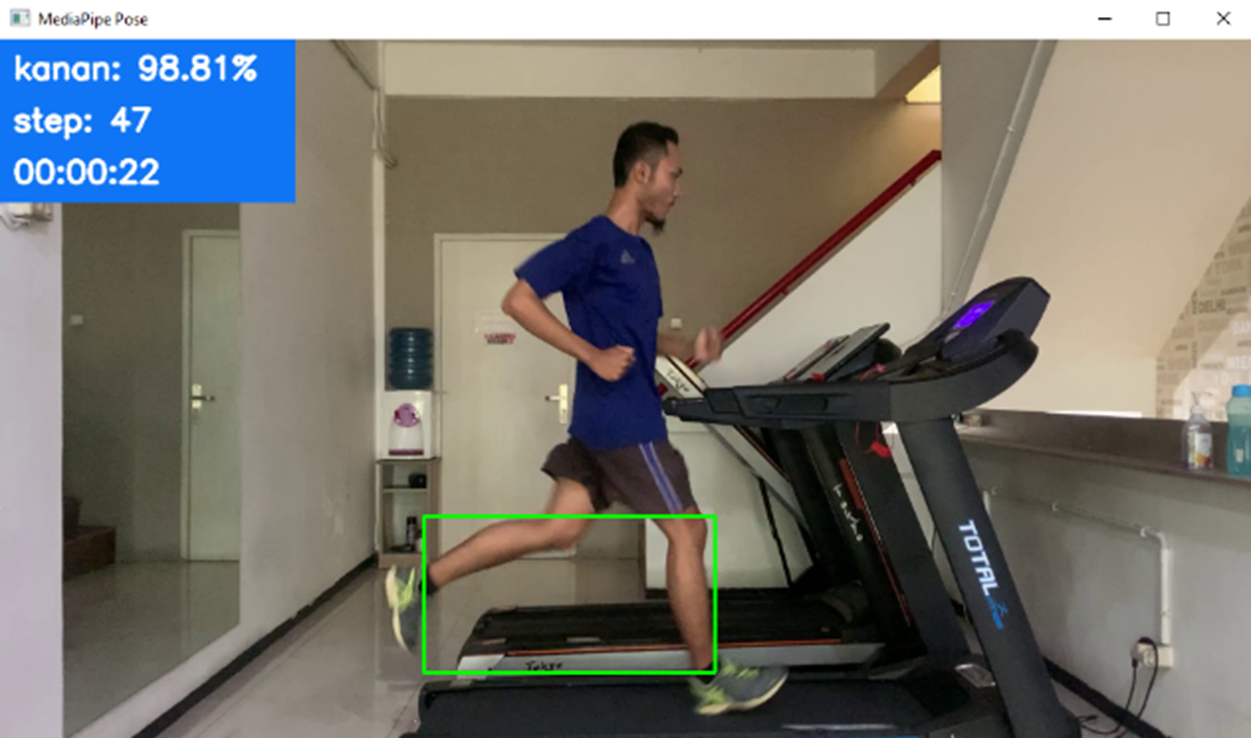
\includegraphics[scale=0.8]{gambar/klasifikasi kanan.png}
  \caption{Klasifikasi untuk kelas kanan}
  \label{fig:KlasifikasiKanan}
\end{figure}

\begin{figure}[H]
  \centering
  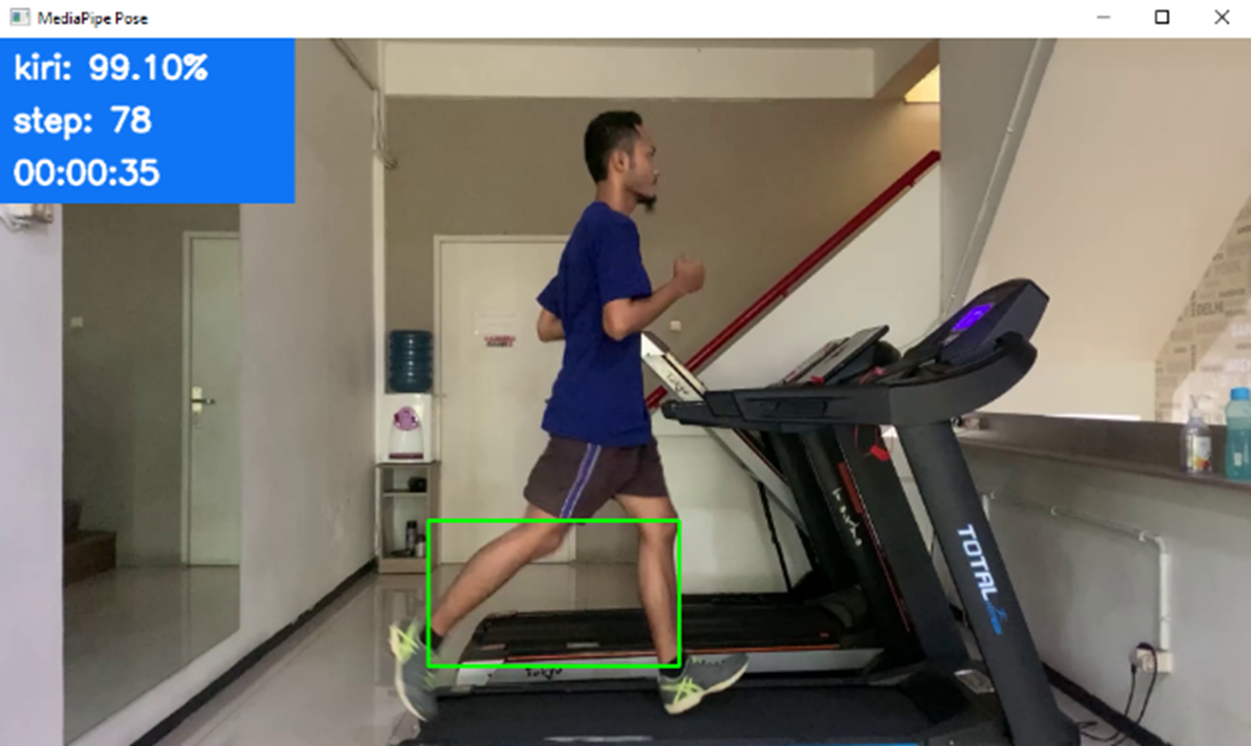
\includegraphics[scale=0.8]{gambar/klasifikasi kiri.png}
  \caption{Klasifikasi untuk kelas kiri}
  \label{fig:KlasifikasiKiri}
\end{figure}


\subsection{Hasil Deteksi}
\label{subsec:HasilDeteksi}

Bentuk hasil klasifikasi yang dibuat adalah mendeteksi pose aktivitas dengan dapat menghitung langkah dan waktu yang ditempuh. Nilai langkah dan waktu yang ditempuh akan digunakan dalam perhitungan selanjutnya. Banyaknya jumlah langkah yang didapat saat hasil deteksi digunakan sebagai nilai variable pertama yang akan digunakan dalam penentuan perhitungan kalori. Langkah dideteksi dan dihitung seberapa banyak langkah yang dilakukan saat proses deteksi. Waktu tempuh saat proses deteksi merupakan nilai variabel kedua yang akan digunakan dalam penentuan perhitungan kalori. Waktu tempuh dimulai saat dideteksi pertama kali nilai langkah yang ditemukan hingga saat akhir langkah tidak ada penambahan kembali yang menandakan proses deteksi telah selesai. Hasil deteksi akan ditampilkan seiring dengan proses deteksi yang dilakukan pada data citra seperti pada Gambar \ref{fig:HasilDeteksi} dan pada akhir proses deteksi akan menampilkan hasil akumulasi akhir dari hasil deteksi terhadap deteksi langkah dan waktu tempuh. Selain itu juga terdapat tampilan hasil perhitungan dan prediksi yang diharapkan dalam penelitian ini. Hasil tampilan untuk hasil deteksi di akhir sebagai akumulasi deteksi ditunjukkan pada Gambar \ref{fig:HasilDeteksi2}.

\begin{figure}[H]
  \centering
  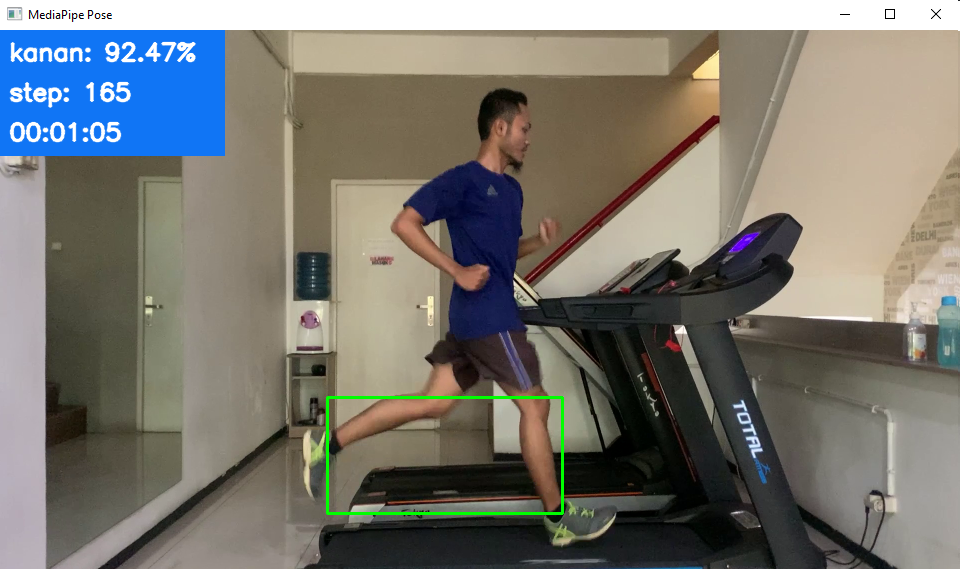
\includegraphics[scale=0.48]{gambar/hasil deteksi.png}
  \caption{Tampilan hasil deteksi saat proses deteksi}
  \label{fig:HasilDeteksi}
\end{figure}

\begin{figure}[H]
  \centering
  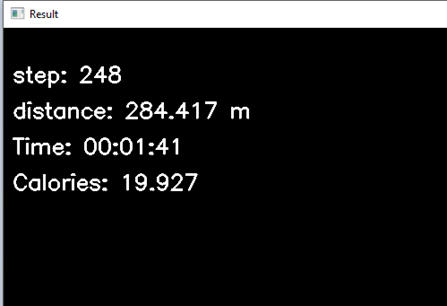
\includegraphics[scale=0.7]{gambar/hasil deteksi2.png}
  \caption{Tampilan akumulasi hasil deteksi}
  \label{fig:HasilDeteksi2}
\end{figure}

\subsection{Hasil Deteksi Langkah}
\label{subsec:HasilLangkah}

Banyaknya jumlah langkah yang didapat saat hasil deteksi digunakan sebagai nilai variable pertama yang akan digunakan dalam penentuan perhitungan kalori. Langkah dideteksi dan dihitung seberapa banyak langkah yang dilakukan saat proses deteksi. Dalam proses deteksi menggunakan model yang sudah dibuat mendapatkan hasil deteksi sesuai kelas yang digunakan yaitu kanan dan kiri. Saat sistem berhasil mendeteksi langkah berdasarkan model langkah kanan dan kiri akan melakukan akumulasi perhitungan langkah dengan menjumlahkan banyak hasil deteksi saat mengalami perubahan hasil deteksi. Dengan adanya perubahan hasil deteksi dari kelas kanan menjadi kiri ataupun sebaliknya, maka sistem akan melakukan penjumlahan pada variabel jumlah langkah berdasarkan hasil deteksi yaitu langkah dengan menggunakan deteksi langkah dari model yang telah dibuat. Saat dideteksinya awal langkah dan perubahan langkah yang mengakibatkan bertambahnya jumlah akumulasi langkah yang dideteksi akan membuat sistem berjalan dan membuat waktu tempuh dimulai berdasarkan hasil langkah awal yang dapat dideteksi. Proses deteksi langkah akan dimulai dengan dimulainya akuisisi data maupun berdasarkan dari data citra dataset dan diakhiri dengan akhir dari deteksi langkah yang tidak mengalami pertambahan dalam kurung waktu tertentu. Hasil akumulasi jumlah langkah akan disimpan dan dilakukan proses selanjutnya dalam menentukan prediksi dan perhitungan kalori.

\subsection{Hasil Waktu Tempuh}
\label{subsec:HasilWaktu}

Waktu tempuh saat proses deteksi merupakan nilai variabel kedua yang akan digunakan dalam penentuan perhitungan kalori. Waktu tempuh dimulai saat dideteksi pertama kali nilai langkah yang ditemukan hingga saat akhir langkah tidak ada penambahan kembali yang menandakan proses deteksi telah selesai. Nilai waktu yang akan digunakan selanjutnya merupakan nilai waktu dalam bentuk satuan detik hasil dari akumulasi keseluruhan dalam proses deteksi. Pada tampilan hasil deteksi waktu tempuh ditampilkan dalam keseluruhan satuan waktu berupa jam, menit dan detik yang dapat dilakukan akumulasi berdasarkan proses melakukan deteksi dari hasil akuisisi data maupun berdasarkan dari data citra dataset. Hasil akumulasi dari satuan detik yang didapat akan disimpan dan dilakukan pada proses selanjutnya dalam menentukan prediksi dan perhitungan kalori.

\section{Prediksi Kalori}
\label{sec:PrediksiKalori}

Prediksi kalori dilakukn dengan dua metode, yaitu menggunakan metode regresi linear dan menggunakan perhitungan rumus EC (Exercise Calories) berdasarkan satuan ukuran MET (Metabolic Equivalent). Kedua metode prediksi ini digunakan sebagai pembanding dalam melakukan analisa terhadap hasil yang didapatkan dari metode prediksi menggunakan metode regresi linear dengan perhitungan rumus. Data yang digunakanan dalam proses prediksi kalori diambil berdasarkan hasil klasifikasi dan hasil deteksi yang telah dilakukan sebelumnya. Hasil deteksi berupa banyaknya langkah dan waktu tempuh digunakan untuk proses prediksi kalori baik dengan metode regresi linear maupun metode perhitungan rumus.

\subsection{Regresi Linear}
\label{subsec:PrediksiRegresi}

Prediksi kalori dengan regresi linear dilakukan dengan teknik analisis untuk mengidentifikasi relasi antar dua variabel atau lebih. Pada penelitian ini varibel yang digunakan adalah hasil deteksi berupa hasil jumlah deteksi langkah dengan hasil waktu tempuh untuk nantinya akan dicari terkait relasi antara variabel tersebut untuk bisa menentukan hasil yang diinginkan yaitu prediksi kalori. Dalam memulai melakukan proses regresi linear untuk prediksi kalori, dilakukan proses pengambilan data untuk diolah menjadi dataset yang akan digunakan dalam beberapa proses pada prediksi kalori dengan regresi linear ini. Proses pengambilan data dilakukan pada alat treadmill yang dilakukan uji dengan beragam variasi dan dilakukan pencatatan data untuk digunakan sebagai dataset pada penelitian ini. Data yang diambil untuk dilakukan pengolahan dari alat treadmill adalah data waktu, kecepatan dan kalori terbakar. Data yang diperoleh dengan mengumpulkan data untuk model regresi linear dari alat treadmill didapatkan jumlah 1045 total data yang dapat dilihat pada Tabel \ref{tb:DatasetRegresi}

\begin{longtable}{|c|c|c|c|}
  \caption{Hasil pengambilan data pada treadmill}
  \label{tb:DatasetRegresi}                                   \\
  \hline
  \rowcolor[HTML]{C0C0C0}
  \textbf{No} & \textbf{Waktu} & \textbf{Kecepatan} & \textbf{Kalori Terbakar} \\
  \hline
  1   & 0:06    & 1 (km/j)    & 0,1     \\
  \hline
  2   & 0:11    & 1 (km/j)    & 0,2     \\
  \hline
  54   & 0:50    & 2 (km/j)    & 1,9     \\
  \hline
  55   & 0:53    & 2 (km/j)    & 2,0     \\
  \hline
  215   & 1:03    & 3 (km/j)    & 3,6     \\
  \hline
  216   & 1:05    & 3 (km/j)    & 3,7     \\
  \hline
  375   & 1:18    & 4 (km/j)    & 6,0     \\
  \hline
  376   & 1:19    & 4 (km/j)    & 6,1     \\
  \hline
  700   & 1:43    & 8 (km/j)    & 16,0     \\
  \hline
  701   & 1:44    & 8 (km/j)    & 16,2     \\
  \hline
  1044   & 2:26    & 12 (km/j)    & 34,1     \\
  \hline
  1045   & 2:27    & 12 (km/j)    & 34,4     \\
  \hline
\end{longtable}

Untuk dapat melakukan prediksi kalori dari hasil deteksi yang didapat menggunakan regresi linear diperlukan model regresi berdasarkan pemodelan dataset yang dibuat terlebih dahulu dan nantinya saat model regresi telah didapat maka akan dapat melakukan prediksi kalori berdasarkan akuisisi maupun dataset untuk dilakukan proses prediksi dengan regresi linear. Dalam melakukan prediksi kalori dengan melakukan pemodelan regresi dilakukan dengan beberapa tahap untuk memproses hasil deteksi sehingga dapat melakukan prediksi. Tahapan untuk membuat model regresi yang diinginkan sesuai model sistem pada penelitian ini adalah dengan membuat regresi jarak tempuh, dataset regresi prediksi kalori dan model regresi linear prediksi kalori.

Tahap pertama dalam melakukan prediksi kalori dari hasi deteksi yang sudah didapat diperlukan untuk melakukan pengolahan data dari hasil deteksi menjadi suatu variabel yang dapat digunakan dalam membuat model regresi. Hasil deteksi berupa banyak langkah dan waktu tempuh diolah agar dapat menjadi variabel dalam membuat model regresi prediksi kalori yang nantinya akan mempermudah dalam data yang didapat saat akuisisi dari hasil deteksi yaitu jarak tempuh dan waktu tempuh. Jarak tempuh pada model regresi prediksi kalori ini didapatkan dengan menggunakan rumus mencari jarak berdasarkan waktu dan kecepatannya yang ditunjukkan pada Persamaan \ref{eq:JarakTempuh}

\begin{equation}
  \label{eq:JarakTempuh}
  Jarak \; Tempuh = Kecepatan \times Waktu
\end{equation}

Dengan menggunakan rumus jarak tempuh berdasarkan kecepatan dan waktu, maka data yang telah dilakupan pengumpulan data untuk regresi linear pada alat treadmil dapat dilakukan pengolahan pada data kecepatan untuk menggunakan jarak tempuh agar mempermudah dalam proses sistem untuk mengenali data berdasarkan hasil deteksi pada penelitian ini. Dari setiap data yang dilakukan pengumpulan data dengan jumlah total data sebanyaka 1045 data akan dilakukan pengolahan untuk nantinya akan menggunakan data waktu tempuh dalam satuan detik, jarak tempuh dalam meter dan kalori yang terbakar. Menentukan jarak tempuh dalam meter dengan menggunakan data berupa waktu dengan satuan menit dan detik lalu kecepatan dalam satuan kilometer per jam dapat melakukan konversi satuan nilai dan menghasilkan persamaan untuk mengubah nilai tersebut sesuai yang diinginkan dan ditunjukkan pada Persamaan \ref{eq:KonversiJarakTempuh}

\begin{equation}
  \label{eq:KonversiJarakTempuh}
  Jarak \; Tempuh \; (meter) = Kecepatan \; (km/j) \times 0,277778 \times Waktu \; (detik)
\end{equation}

Data yang telah dilakukan pengumpulan data pada alat treadmill kemudian dilakukan pengolahan data untuk memudahkan dalam penyesuaian data pada sistem. Dengan menggunakan perubahan data dengan persamaan konversi untuk mencari jarak tempuh, didapat data baru yang telah dilakukan pengolahan data. Tabel \ref{tb:OlahDatasetRegresi} menunjukkan data terbaru setelah melakukan pengolahan data dari proses pengambilan data. 

\begin{longtable}{|c|c|c|c|}
  \caption{Hasil pengolahan data pada dataset kalori}
  \label{tb:OlahDatasetRegresi}                                   \\
  \hline
  \rowcolor[HTML]{C0C0C0}
  \textbf{No} & \textbf{Waktu (detik)} & \textbf{Jarak Tempuh (meter)} & \textbf{Kalori Terbakar} \\
  \hline
  1   & 6    & 1.666668    & 0,1     \\
  \hline
  2   & 11    & 3.055558    & 0,2     \\
  \hline
  54   & 50    & 27.7778    & 1,9     \\
  \hline
  55   & 53    & 29.444468    & 2,0     \\
  \hline
  215   & 63    & 52.500042    & 3,6     \\
  \hline
  216   & 65    & 54.16671    & 3,7     \\
  \hline
  375   & 78    & 86.666736    & 6,0     \\
  \hline
  376   & 79    & 87.777848    & 6,1     \\
  \hline
  700   & 103    & 226.666848    & 16,0     \\
  \hline
  701   & 104    & 228.889072    & 16,2     \\
  \hline
  1044   & 146    & 486.667056    & 34,1     \\
  \hline
  1045   & 147    & 490.000392    & 34,4     \\
  \hline
\end{longtable}

Hasil pengolahan data pada dataset dilanjutkan dengan melakukan pembuatan model regresi linear dari dataset yang telah dibuat untuk dapat melakukan prediksi kalori terbakar. Model regresi linear dibuat berdasarkan data berupa waktu dalam detik, jarak tempuh dalam meter dan kalori yang terbakar dalam kcal berdasarkan data pada treadmill yang sudah dilakukan pengambilan data dan pengolahan data. Pada model regresi linear dibutuhkan dua variabel yaitu variabel independen dan variabel dependen. Dataset yang telah didapat dilakukan pembagian berdasarkan variabel yang diperlukan berdasarkan model regresi yang diinginkan. Variabel independen dari dataset mencakup data mengenai waktu dan jarak tempuh, sedangkah variabel dependen dari dataset mencakup data kalori terbakar. Berdasarkan pembagian dataset kalori sesuai variabel regresi yang dibuat kemudian akan dilakukan pembuatan model regresi dalam persamaan regresi linear. Tabel \ref{tb:VariabelPrediksiKalori} menunjukkan pembagian dataset berdasarkan variabel untuk model regresi yang akan dilakukan. 

\begin{longtable}{|c|c|c|}
  \caption{Pembagian dataset kalori berdsarkan variabel regresi}
  \label{tb:VariabelPrediksiKalori}                                   \\
  \hline
  \rowcolor[HTML]{C0C0C0}
  \multicolumn{2}{|c|}{\textbf{Variabel Independen}}  & \textbf{Variabel Dependen}  \\
  \hline
  \rowcolor[HTML]{C0C0C0}
  \textbf{Waktu (detik)} & \textbf{Jarak Tempuh (meter)} & \textbf{Kalori Terbakar} \\
  \hline
  6    & 1.666668    & 0,1     \\
  \hline
  11    & 3.055558    & 0,2     \\
  \hline
  50    & 27.7778    & 1,9     \\
  \hline
  53    & 29.444468    & 2,0     \\
  \hline
  63    & 52.500042    & 3,6     \\
  \hline
  65    & 54.16671    & 3,7     \\
  \hline
  78    & 86.666736    & 6,0     \\
  \hline
  79    & 87.777848    & 6,1     \\
  \hline
  103    & 226.666848    & 16,0     \\
  \hline
  104    & 228.889072    & 16,2     \\
  \hline
  146    & 486.667056    & 34,1     \\
  \hline
  147    & 490.000392    & 34,4     \\
  \hline
\end{longtable}

Model regresi linear dibuat berdasarkan pembagian dataset sesuai variabel yang digunakan. Setelah pembagian dataset telah dilakukan, pembuatan model regresi linear dilakukan dengan memahami pola dari data variabel independen untuk menghasilkan variabel dependen. Pembuatan model regresi dilakukan dengan menganalisa dari setiap kemungkinan yang akan terjadi berdasarkan variabel independen untuk bisa memperkirakan hasil yang diinginkan berdasarkan variabel dependen. Analisa yang dilakukan untuk membuat model regresi mendapatkan model persamaan yang nantinya dapat digunakan untuk melakukan pada data akuisisi baru. Hasil dari model regresi linear berupa persamaan regresi linear yang akan digunakan dalam proses prediksi selanjutnya. Dataset yang telah dibagi dilakukan prose pembuatan model menghasilkan model persamaan regresi linear yang akan digunakan dalam menentukan nilai prediksi kalori yang terbakar. Persamaan yang didapatkan dari model regresi linear dari dataset kalori ditunjukkan pada Persamaan \ref{eq:PersamaanRegresiKalori}.

\begin{equation}
  \label{eq:PersamaanRegresiKalori}
  Kalori \; Terbakar = - \; 0.00030418 \times Waktu + 0.0704 \times Jarak - 0.06703071381901893 \; kkal
\end{equation}

Persamaan dari model regresi yang didapat digunakan untuk melakukan prediksi kalori yang terbakar setelah mendapatkan data hasil prediksi yang akan diproses untuk dapat menjadi data yang diperlukan pada persamaan model regresi prediksi kalori. Pada persmaan model regresi didapatkan untuk melakukan prediksi kalori memerlukan data waktu dan jarak tempuh sesuai dengan dataset kalori. Satuan yang didapat pada persamaan berupa kalori yang terbakar dengan satuan berupa kcal. Saat melakukan akuisisi data akan dilakukan proses untuk mendapatkan data yang dapat digunakan dalam persamaan model regresi linear ini. Hasil dari proses pada data akuisisi akan digunakan pada persamaan model regresi linear untuk nantinya akan mendapatkan hasil prediksi kalori dengan model regresi yang digunakan. Dataset yang telah dilakukan pembuatan persamaan model regresi dapat dilakukan pembuatan proyeksi model regresi berdasarkan data dan persamaan regresi linear yang digunakan. Hasil proyeksi dari model regresi linear untuk prediksi kalori terbakar yang didapatkan ditunjukkan pada Gambar \ref{fig:ModelRegresiKalori}.

\begin{figure}[H]
  \centering
  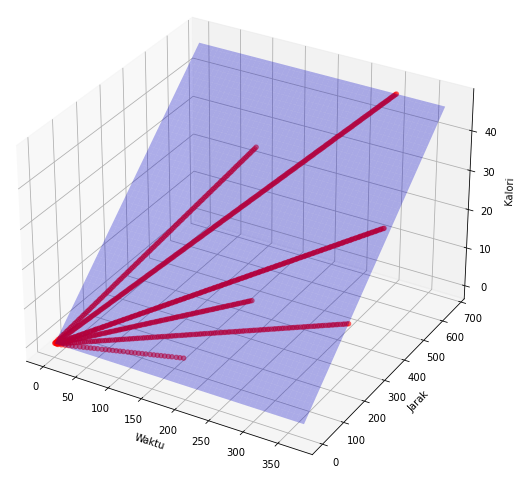
\includegraphics[scale=0.7]{gambar/model regresi kalori3.png}
  \caption{Model regresi linear prediksi kalori terbakar}
  \label{fig:ModelRegresiKalori}
\end{figure}

Tahap selanjutnya setelah mendapatkan model regresi linear untuk prediksi kalori terbakar adalah perhitungan banyak langkah berdasarkan dataset yang telah dibuat dengan mengamati perhitungan langkah dari data video sebenarnya. Data banyak langkah ini akan digunakan sebagai acuan dalam menentukan panjang langkah yang dihasilkan dari tiap variasi yang dilakukan. Dalam melangkah seseorang akan menghasilkan panjang langkah yang berbeda berdasarkan kecepatan yang dilakukan. Panjang langkah ini akan digunakan sebagai pengali dari data akuisisi berupa banyak langkah untuk nantinya dapat menghasilkan jarak tempuh yang dilakukan. Untuk menentukan panjang langkah yang didapat berdasarkan data jarak tempuh dan banyak langkah yang ditempuh dapat dengan menggunakan konversi persamaan yang ditunjukkan pada Persamaan \ref{eq:KonversiPanjangLangkah}.

\begin{equation}
  \label{eq:KonversiPanjangLangkah}
  Panjang \; Langkah = \frac{Jarak \; Tempuh}{Banyak \; Langkah}
\end{equation}

Proses perhitungan banyak langkah dari data video yang digunakan disimpan menjadi dataset untuk selanjutnya dilakukan pengolahan data. Hasil dataset perhitungan banyak langkah juga dilanjutkan dengan perhitungan panjang langkah dari setiap variasi dataset. Proses ini dilakukan untuk membuat dataset yang nantinya akan digunakan untuk melakukan prediksi terhadap panjang langkah saat melakukan estimasi pose dan deteksi langkah. Prediksi panjang langkah ini digunakan sebelum melakukan proses prediksi kalori terbakar saat melakukan akuisisi data dan prediksi kalori terbakar untuk mendapatkan data jarak tempuh yang kemudian digunakan untuk melakukan prediksi kalori terbakar. Tabel \ref{tb:OlahDatasetPanjang} menunjukkan hasil pengolahan data untuk dataset panjang langkah yang akan dilakukan pada proses prediksi panjang langkah.

\begin{longtable}{|c|c|c|c|}
  \caption{Hasil pengolahan data pada dataset panjang langkah}
  \label{tb:OlahDatasetPanjang}                                   \\
  \hline
  \rowcolor[HTML]{C0C0C0}
  \textbf{No} & \textbf{Waktu (detik)} & \textbf{Langkah} & \textbf{Panjang Langkah} \\
  \hline
  1   & 6    & 4    & 0.38089      \\
  \hline
  2   & 11    & 8    & 0.38089     \\
  \hline
  54   & 50    & 53    & 0.52057     \\
  \hline
  55   & 53    & 57    & 0.52057     \\
  \hline
  215   & 63    & 85    & 0.61583     \\
  \hline
  216   & 65    & 88    & 0.61583     \\
  \hline
  375   & 78    & 131    & 0.66120     \\
  \hline
  376   & 79    & 133    & 0.66120     \\
  \hline
  700   & 103    & 263    & 0.86869     \\
  \hline
  701   & 104    & 266    & 0.86869     \\
  \hline
  1044   & 146    & 385    & 1.26289     \\
  \hline
  1045   & 147    & 388    & 1.26289     \\
  \hline
\end{longtable}

Hasil pengolahan data untuk dataset panjang langkah digunakan untuk membuat model regresi polinomial dalam menentukan prediksi panjang langkah. Model regresi polinomial dibuat berdasarkan data berupa waktu dalam detik, langkah dan panjang langkah. Pembagian data dilakukan berdasarkan variabel dalam membuat model regresi polinomial yaitu variabel independen dan variabel dependen. Variabel independen mencakup data mengenai waktu dan langkah, sedangkan variabel dependen merupakan data panjang langkah. Tabel \ref{tb:VariabelPrediksiPanjang} menunjukkan pembagian dataset berdasarkan variabel untuk model regresi yang akan dilakukan.

\begin{longtable}{|c|c|c|}
  \caption{Pembagian dataset panjang langkah berdsarkan variabel regresi}
  \label{tb:VariabelPrediksiPanjang}                                   \\
  \hline
  \rowcolor[HTML]{C0C0C0}
  \multicolumn{2}{|c|}{\textbf{Variabel Independen}}  & \textbf{Variabel Dependen}  \\
  \hline
  \rowcolor[HTML]{C0C0C0}
  \textbf{Waktu (detik)} & \textbf{Langkah} & \textbf{Panjang Langkah} \\
  \hline
  6    & 4    & 0.38089      \\
  \hline
  11    & 8    & 0.38089     \\
  \hline
  50    & 53    & 0.52057     \\
  \hline
  53    & 57    & 0.52057     \\
  \hline
  63    & 85    & 0.61583     \\
  \hline
  65    & 88    & 0.61583     \\
  \hline
  78    & 131    & 0.66120     \\
  \hline
  79    & 133    & 0.66120     \\
  \hline
  103    & 263    & 0.86869     \\
  \hline
  104    & 266    & 0.86869     \\
  \hline
  146    & 385    & 1.26289     \\
  \hline
  147    & 388    & 1.26289     \\
  \hline
\end{longtable}

Model regresi polinomial dibuat berdasarkan pembagian dataset sesuai variabel yang digunakan. Hasil dari model regresi polinomial berupa persamaan regresi polinomial yang akan digunakan dalam proses prediksi selanjutnya. Dataset yang telah dibagi dilakukan prose pembuatan model menghasilkan proyeksi model regresi berdasarkan data dan persamaan regresi polinomial yang digunakan. Hasil proyeksi dari model regresi polinomial untuk prediksi panjang langkah yang didapatkan ditunjukkan pada Gambar \ref{fig:ModelRegresiPanjang}.

\begin{figure}[H]
  \centering
  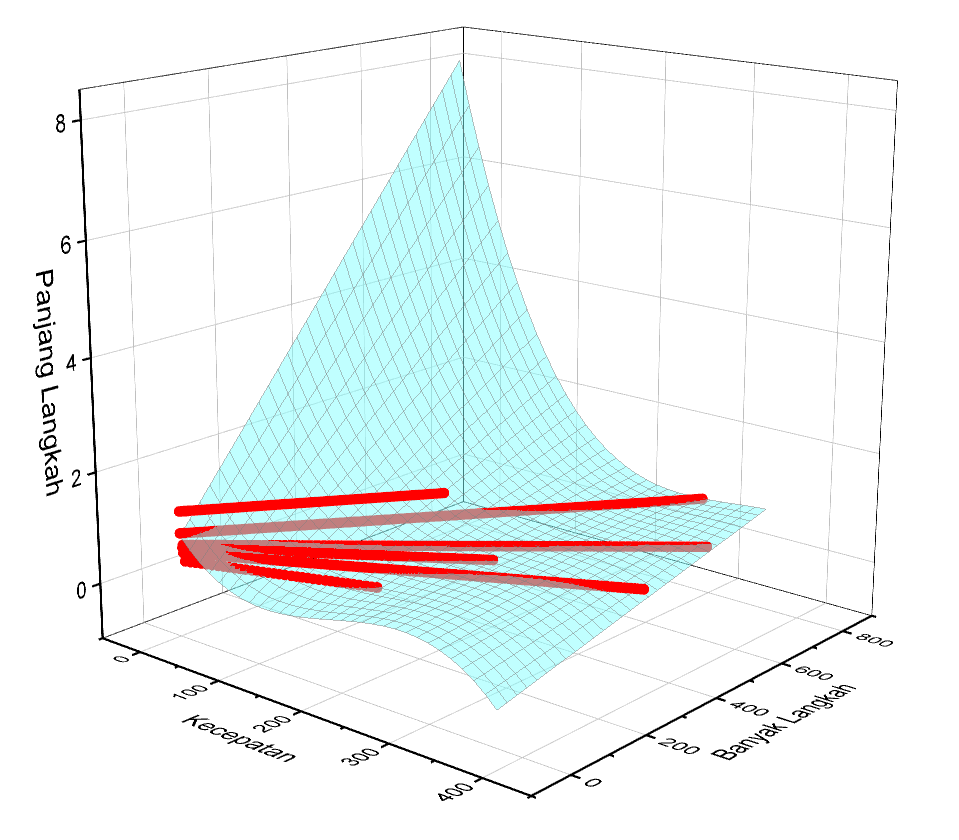
\includegraphics[scale=0.5]{gambar/model regresi panjang.png}
  \caption{Model regresi polinomial prediksi panjang langkah}
  \label{fig:ModelRegresiPanjang}
\end{figure}

Setelah pengolahan data dan model telah dilakukan dapat dilanjutkan dengan melakukan proses prediksi kalori yang terbakar dengan regresi linear. Proses melakukan prediksi dapat dilakukan dengan melakukan akuisisi data dengan data video atau menggunakan pengambilan data secara langsung. Data video kemudian dilanjutkan dengan proses estimasi pose untuk mendapatkan beberapa data gambar yang akan digunakan untuk proses klasifikasi dengan model deteksi langkah. Saat klasifikasi akan menghasilkan data yang nantinya akan digunakan untuk prediksi kalori. Hasil klasifikasi berupa data banyak langkah dan waktu tempuh. Data hasil klasifikasi akan diproses untuk dicari panjang langkah dengan model regresi polinomial untuk prediksi panjang langkah. Hasil prediksi akan digunakan untuk melakukan perhitungan terhadap banyak akumulasi langkah dikalikan dengan prediksi panjang langkah untuk menghasilkan jarak tempuh. Setelah didapatkan jarak tempuh dan waktu tempuh saat akuisisi data sudah dilakukan akan dilanjutkan dengan prediksi kalori menggunakan model regresi linear untuk prediksi kalori terbakar. Hasil prediksi kalori terbakar akan didapatkan berdasarkan model yang sudah dibuat dan data yang didapat.

\subsection{Perhitungan Rumus}
\label{subsec:PrediksiPerhitungan}

Perhitungan kalori dilakukan dengan mengacu pada nilai satuan ukuran \emph{(Metabolic Equivalent of Task)} (MET). Satuan MET akan mendapat pengukuran untuk konsumsi oksigen dan pembakaran kalori. Nilai dari satuan MET dapat didefinisikan dengan nilai 1 MET setara dengan 3,5 mL O\textsubscript{2}/kg/menit. Diketahui juga dalam konsumsi oksigen dengan nilai 1.000 mL setara dengan pembakaran energi sebesar 5 kkal. Berdasarkan nilai satuan ukuran MET dan pembakaran energi, didapatkan suatu persamaan untuk menghitung pembakaran kalori yang didefiniskan pada Persamaan \ref{eq:RumusKalori1}.

\setcounter{chapter}{2}
\setcounter{equation}{0}
\begin{equation}
  Kalori \; Terbakar = \frac{MET \times 3.5 \times berat \; badan \; (kg)}{200} \; kkal/menit
\end{equation}
\setcounter{chapter}{3}
\setcounter{equation}{4}

Pada persamaan pembakaran kalori yang akan digunakan untuk melakukan perhitungan pembakaran kalori dari aktivitas yang dilakukan dibutuhkan beberapa nilai variabel untuk mendapatkah hasil total pembakaran kalori, yaitu nilai MET, nilai berat badan dalam kilogram (kg), dan nilai waktu tempuh dalam menit.

Setiap aktivitas memiliki nilai MET yang berbeda-beda dan telah ditentukan oleh peneliti yang telah merangkum banyak aktivitas untuk ditentukan berapa nilai MET yang dihasilkan berdasarkan beberapa jenis yang telah ditunjukkan pada Tabel \ref{tb:metjenisaktivitas}. Pada aktivitas olahraga yang difokuskan saat ini adalah jogging pada treadmill juga memiliki perbedaan nilai MET yang dipengaruhi oleh kecepatan jogging. Dataset MET terkait aktivitas olaharga terhadap jogging didapatkan berdasarkan penelitian oleh Ainsworth pada \emph{Compendium of Physical Activities} (\ref{subsec:compendium}) untuk digunakan dalam prediksi kalori terbakar menggunakan perhitungan rumus pada penelitian ini. Terdapat data variasi kecepatan yang memiliki nilai MET yang bervariasi. Tabel \ref{tb:DatasetMET} menunjukkan dataset yang digunakan sebagai acuan dalam menentukan kecepatan dan MET yang didapat untuk kemudian dilakukan proses prediksi kalori terbakar.

\begin{longtable}{|c|c|}
  \caption{Dataset pengaruh kecepatan terhadap MET}
  \label{tb:DatasetMET}                                   \\
  \hline
  \rowcolor[HTML]{C0C0C0}
  \textbf{Kecepatan (km/j)} & \textbf{MET}  \\
  \hline
  6.43738  & 6    \\
  \hline
  8.04672   & 8.3    \\
  \hline
  8.36859   & 9    \\
  \hline
  9.65606   & 9.8    \\
  \hline
  10.7826   & 10.5    \\
  \hline
  11.2654   & 11    \\
  \hline
  12.0701   & 11.8    \\
  \hline
  12.8748   & 11.8    \\
  \hline
  13.8404   & 12.3    \\
  \hline
  14.4841   & 12.8    \\
  \hline
  16.0934   & 14.5    \\
  \hline
  17.7028   & 16    \\
  \hline
  19.3121   & 19    \\
  \hline
  20.9215   & 19.8    \\
  \hline
  22.5308   & 23    \\
  \hline
\end{longtable}

Dataset MET yang didapat menunjukkan jika nilai MET dapat diketahui dengan berdasarkan kecepatan yang dilakukan saat melakukan aktivitas olahraga \emph{jogging}. Berdasarkan hasil deteksi pada sistem yang digunakan pada penelitian ini untuk melakukan prediksi kalori berupa jumlah langkah dan waktu tempuh yang kemudian dilakukan pengolahan data untuk menghasilkan data jarak tempuh dan waktu tempuh dapat dilakukan pengolahan lanjut untuk mencari kecepatan tempuh. Kecepatan tempuh dapat kemudian dilakukan pengolahan kembali untuk mencari nilai MET dan melakukan prediksi kalori terbakar dengan menggunakan rumus. Untuk mencari kecepatan tempuh dapat diketahui dengan nilai hasil deteksi dan pengolahan data berupa jarak tempuh dan waktu tempuh untuk menentukan kecepatan tempuh dengan menggunakan Persamaan \ref{eq:RumusKecepatan}.

\begin{equation}
  \label{eq:RumusKecepatan}
  Kecepatan = \frac{Jarak}{Waktu}
\end{equation}

Berdasarkan dataset kecepatan untuk mengetahui MET dapat kemudian dilakukan pembuatan model regresi polinomial untuk dapat menentukan prediksi MET berdasarkan hasil deteksi dengan pengolahan berupa data kecepatan. Model regresi polinomial dibuat berdasarkan data berupa kecepatan dan MET. Pembagian data dilakukan berdasarkan variabel dalam membuat model regresi polinomial yaitu variabel independen dan variabel dependen. Variabel independen meliputi data kecepatan dan variabel dependen meliputi data MET. Tabel \ref{tb:VariabelPrediksiMET} menunjukkan pembagian dataset berdasarkan variabel untuk model regresi yang akan dilakukan.

\begin{longtable}{|c|c|}
  \caption{Pembagian dataset MET berdasarkan variabel regresi}
  \label{tb:VariabelPrediksiMET}                                   \\
  \hline
  \rowcolor[HTML]{C0C0C0}
  \textbf{Variabel Independen}  & \textbf{Variabel Dependen}  \\
  \hline
  \rowcolor[HTML]{C0C0C0}
  \textbf{Kecepatan (km/j)} & \textbf{MET}  \\
  \hline
  6.43738  & 6    \\
  \hline
  8.04672   & 8.3    \\
  \hline
  8.36859   & 9    \\
  \hline
  9.65606   & 9.8    \\
  \hline
  10.7826   & 10.5    \\
  \hline
  11.2654   & 11    \\
  \hline
  12.0701   & 11.8    \\
  \hline
  12.8748   & 11.8    \\
  \hline
  13.8404   & 12.3    \\
  \hline
  14.4841   & 12.8    \\
  \hline
  16.0934   & 14.5    \\
  \hline
  17.7028   & 16    \\
  \hline
  19.3121   & 19    \\
  \hline
  20.9215   & 19.8    \\
  \hline
  22.5308   & 23    \\
  \hline
\end{longtable}

Model regresi polinomial dibuat berdasarkan pembagian dataset sesuai variabel yang digunakan. Hasil dari model regresi polinomial berupa persamaan regresi polinomial yang akan digunakan dalam proses prediksi selanjutnya. Dataset yang telah dibagi dilakukan prose pembuatan model menghasilkan proyeksi model regresi berdasarkan data dan persamaan regresi polinomial yang digunakan. Hasil proyeksi dari model regresi polinomial untuk prediksi MET yang didapatkan ditunjukkan pada Gambar \ref{fig:ModelRegresiMET}.

\begin{figure}[H]
  \centering
  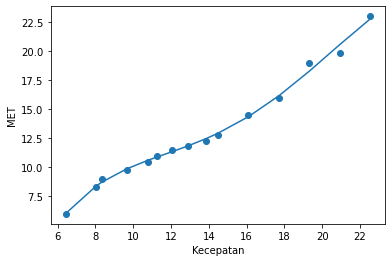
\includegraphics[scale=0.8]{gambar/model regresi poli met.png}
  \caption{Model regresi polinomial prediksi MET}
  \label{fig:ModelRegresiMET}
\end{figure}

Setelah pengolahan data dan model telah dilakukan dapat dilanjutkan dengan melakukan proses prediksi kalori yang terbakar dengan perhitungan rumus. Proses melakukan prediksi dapat dilakukan dengan melakukan akuisisi data dengan data video atau menggunakan pengambilan data secara langsung. Data video kemudian dilanjutkan dengan proses estimasi pose untuk mendapatkan beberapa data gambar yang akan digunakan untuk proses klasifikasi dengan model deteksi langkah. Saat klasifikasi akan menghasilkan data yang nantinya akan digunakan untuk prediksi kalori. Hasil klasifikasi berupa data banyak langkah dan waktu tempuh. Data hasil klasifikasi akan diproses untuk dicari panjang langkah dengan model regresi polinomial untuk prediksi panjang langkah. Hasil prediksi akan digunakan untuk melakukan perhitungan terhadap banyak akumulasi langkah dikalikan dengan prediksi panjang langkah untuk menghasilkan jarak tempuh. Setelah didapatkan jarak tempuh dan waktu tempuh saat akuisisi data sudah dilakukan akan dilanjutkan dengan pengolahan data dari hasil deteksi jarak tempuh dan waktu tempuh untuk diketahui kecepatan tempuh berdasarkan konversi pada pengolahan data. Kecepatan tempuh yang didapat akan dilakukan prediksi MET menggunakan model regresi polinomial untuk prediksi MET. Hasil MET yang didapat akan dilakukan perhitungan menggunakan perhitungan rumus berdasarkan MET untuk kemudian menggunakan data waktu tempuh dan variabel berat badan (BB) sebesar 65 sebagai ukuran standar. Perhitungan rumus yang dilakukan berdasarkan nilai-nilai variabel yang telah ditentukan dalam proses merupakan hasil akhir berupa prediksi kalori yang terbakar.
